%-----------------------------------------------------------------------------%
%	Packages & Other Configurations
%-----------------------------------------------------------------------------%
\RequirePackage{fix-cm}  % Fix Font shape `OT1/cmr/m/n' size substitution.
\documentclass[a4paper,10pt]{article}
\usepackage[top=0.5in, bottom=0.6in, left=1in, right=0.9in]{geometry}
\usepackage[utf8]{inputenc} %add acents
\usepackage{setspace} % command \doublespacing etc...
\usepackage{lineno} % number lines
\usepackage{epsf,epsfig} % includegraphics [pdf, png etc]
\usepackage{amsmath} %adicionei esse pacote pra vc poder usar o draft%
\usepackage{textcomp} %símbolos de texto
\usepackage{natbib} % bibtex - adicionar referencia
% \usepackage{url} % for bibtex - configuracoes de urls
\usepackage{tabularx} % for tables
\usepackage[hidelinks]{hyperref}  % Add URL links.
% \usepackage[bookmarks=false,colorlinks=true,urlcolor={green},linkcolor={green},pdfstartview={XYZ null null 1.22}]{hyperref} %all references

%-----------------------------------------------------------------------------%
%	Adicionar a Watermark
%-----------------------------------------------------------------------------%
\usepackage{draftwatermark}
\SetWatermarkAngle{45}
\SetWatermarkLightness{0.9}
\SetWatermarkFontSize{5cm}
\SetWatermarkScale{0.3}
\SetWatermarkText{Exercício - Oceanografia}

%-----------------------------------------------------------------------------%
%	Informações sobre o PDF
%-----------------------------------------------------------------------------%

\pdfinfo{%
  /Title    (GEO232 - Exercício)
  /Author   (Ju Leonel)
  /Creator  (Ju Leonel)
  /Producer (Ju Leonel)
  /Subject  (Intro oceanografias)
  /Keywords (Intro oceanografia, exercício Ondas e Marés)}

%-----------------------------------------------------------------------------%
%	Documento
%-----------------------------------------------------------------------------%
\title{GEO232 - Introdução à Oceanografia - IGEO-UFBA}
\author{\vspace{-10ex}}
\date{\vspace{-10ex}}

\begin{document}

  \maketitle
  %\doublespacing
  \onehalfspace

  \begin{tabular*} {0.9\textwidth}{@{\extracolsep{\fill} } l l}
    \hline
    Professora: Juliana Leonel & Atendimento: Sextas-feiras \\
    E-mail: \href{mailto:jleonel@ufba.br}{jleonel@ufba.br} & Horário atendimento: 13:00-14:00 \\
    Aulas: Terças e Quintas-Feiras & Local atendimento: IGEO - Sala 10 - 2\textsuperscript{o} andar\\
    Horário- Aulas: 10:40 - 12:30 & Homepage: \url{http://juoceano.github.io/introductiontooceanography}\\
    \hline
  \end{tabular*}

  \vspace{3ex}

    \section*{Exercício: Ondas e Marés}

    \begin{itemize}
      \item[1)] Faça um paralelo, usando tudo que você sobre ondas em geral, entre
            ondas sonoras, ondas de luz e ondas no mar.  Forneça a sua resposta
            na forma de uma tabela com 3 colunas (usando as ondas acima) e
            quantas linhas você conseguir em sua comparação até um máximo de 10.
%   **Repostas:**
%   - Todas mudam suas propriedades ao mudar o comprimento de ondas: curtas e
%     longas, como mudam a cor, o Som
%   - Luz também se comporta como partícula Som e OM não
%   - Velocidade: Luz > Som > OM
%   - Meio de propagação: Luz ideal no vácuo (mas virtualmente em qualquer meio mas não sólidos!);
%     Som: Não se propaga no vácuo; OM na intarface ar-mar.
      \item[2)] Qual é a relação entre ondas no mar e o vento?
      \item[3)] Porque as ondas no mar chegam sempre "quase" paralelas à praia?
      \item[4)] A maré é uma onda?  E o Tsunami é uma onda?  Explique sua resposta.
      \item[5)] O que você pode dizer sobre a periodicidade das ondas no mar, das
            marés e dos Tsunamis?
      \item[6)] Ondas em alto mar (profundidade maior que 1000 metros) é igual a
            Onda do surfista?  Justifique sua resposta?
      \item[7)] O que é ``ressaca'' no mar?  A onda observada durante uma ressaca é
            diferente da onda observada normalmente?  Elabora as semelhanças e
            diferenças em uma tabela?
      \item[8)] O que você entende por ``onda-interna?''

      \item[9)] Preencha com nomes apropriados as 5 setas indicativas na figura
            abaixo.

            \begin{figure}[h!]
              \centering
              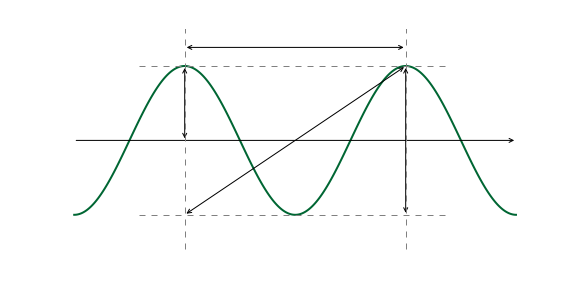
\includegraphics[width=0.95\textwidth]{esquema_ondas_branco}
            \caption{Onda esquemática.}
          \end{figure}
      \item[10)] Marés, se compararmos o mesmo lugar ao longo do tempo
                 (digamos 1-2 meses), podem variar os níveis máximos e mínimos
                 de altura.  Se compararmos lugares diferentes a maré pode mudar
                 sua frequência e suas amplitudes máximas e mínimas.  Quais
                 fatores podem estar relacionados com essa mudança?
      \item[11)] Visite o Museu X e conheça a máquina de previsão de marés do
                 Lord Kelvin.
    \end{itemize}
\end{document}
